% Part 1: Determining RecB binding time
\section*{Results}

\subsection*{RecB forms long-lived spots when recruited to DSBs caused by cipro\-floxacin}
To quantify RecB binding time to DSBs in live \ecoli, we used a Halo-tag fusion to the RecB subunit, conjugated to the JF549 fluorescent dye (Figure \ref{Fig:exp_principle}A). The fusion was previously fully characterised, ensuring specific one-to-one labelling of RecB molecules without adverse effects on the DNA repair process \cite{Lepore2019a,Lepore2023}. As a result of the large size and topological constraints of the bacterial chromosome, DSB-bound RecB diffuses very slowly \cite{Lepore2023}. Therefore, we applied the previously developed technique of localisation enhancement \cite{Yu2006, Elf2007}: since RecB is present at low copy numbers in \ecoli\ [$\sim$5 molecules per cell on average \cite{Lepore2019a,Kalita2024}], imaging live cells with a long exposure time (1 second) made fast-diffusing RecB molecules appear as weak homogeneous signal in the cell, while very slow-diffusing RecB molecules formed diffraction-limited spots (referred to throughout this article as RecB spots, Figures \ref{Fig:exp_principle}B and \ref{Fig:exp_principle}C). The complete absence of similar spots in cells expressing the free Halo-tag from a plasmid confirmed that these spots were specific to RecB (Supp. Figure \ref{SIFig:freehalo_image}). However, their exact nature needed to be confirmed. Although DSB-bound molecules are expected to diffuse very slowly, the RecBCD-Halo complex diffuses in the crowded and constrained environment of the cytoplasm, and might undergo transient interactions with DNA \cite{Lepore2023}, which could lead to RecB spots forming independently of DSB binding. To gain more insight into the nature of RecB spots, we increased the number of DSBs by adding ciprofloxacin to agar pads before imaging, and measured the lifetime of the spots by recording 100-second timelapse videos with 2-sec interval between frames at different positions in the sample, for a total time of 75 min following exposure to ciprofloxacin (Figure \ref{Fig:lifetimes}A). The 1-second exposure time was optimised to detect RecB spots with good signal-to-noise while limiting dye photobleaching and keeping a sufficient temporal resolution to determine spot lifetimes. Visual inspection of the timelapse data showed that RecB spot lifetime was hetereogenous, with a majority of spots being visible only for a 1-2 frames, and a small number persisting for longer times. These longer-lived spots became more frequent as the ciprofloxacin concentration increased. Background-subtracted intensity time-traces for single RecB spots showed that spots lost their intensity in a single step (Supp. Figure \ref{SIFig:SM_traces}), consistent with single-molecule photobleaching or transitioning from a very slowly diffusing state to a rapid one. Therefore, our imaging setup allowed us to visualise single, very slow diffusing RecB molecules, and to measure the time they spent in this diffusive state.

\begin{figure}[htbp]
    \centering
    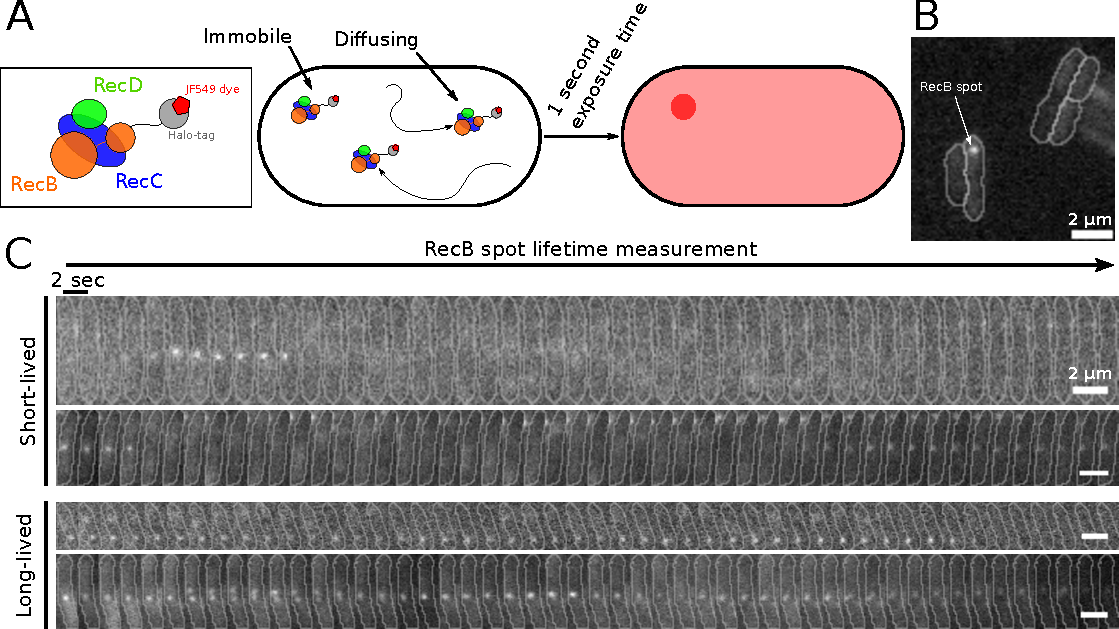
\includegraphics[width=.45\textwidth]{Figures/Fig1_Exp_principle.pdf}
    \caption{Detecting RecB binding to DSBs. \textbf{(A)} Scheme of our experimental protocol. The RecB subunit of the RecBCD complex is fused to a Halo-tag, bound by the JF549 fluorescent dye \cite{Lepore2019a, Lepore2023}. \textbf{(B)} A long exposure time (1 sec) makes diffusing molecules appear as a diffuse signal in the cell, while DSB-bound molecules are visible as bright, diffraction-limited spots. \textbf{(C)} Example image of a RecB spot (white arrow).}
    \label{Fig:exp_principle}
\end{figure}

\subsection*{RecB forms long-lived complexes with DSBs}
% RecB spot lifetime
Using the time-lapse data, we built histograms of RecB spot lifetimes at the different ciprofloxacin concentrations (Figure \ref{Fig:lifetimes}B). In the absence of ciprofloxacin, the majority of spots lasted less than 2 seconds. Under increasing ciprofloxacin concentrations, the distribution showed a clear shift towards longer-lived spots, with the histogram at 20 and 30 ng/ml ciprofloxacin displaying a clear "tail" of long-lived events ($>$ 10 sec). Fitting these histograms with a mono-exponential decay model ($y = a.e^{-k.t}$) did not match the experimental data accurately (Supp. Figure \ref{SIFig:monoexp_fits}). In particular, it did not account for the tail of longer-lived spots that formed at high ciprofloxacin concentrations. Fitting with a bi-exponential decay model ($y = a_1.e^{-k_1.t} + a_2.e^{-k_2.t}$) accounted better for the longer-lived RecB spots (Figure \ref{Fig:lifetimes}B). The bi-exponential fit outlined two populations of spots with different lifetimes: a short-lived one, with average lifetimes ranging from 1.4 to 1.7 sec; and a longer-lived one, with average lifetimes ranging from 10 to 14 sec (Table \ref{tab:fit_results}). Even though the short-lived spots always represented a majority of events (over 90\% of the spots), the proportion of long-lived spots increased under higher ciprofloxacin exposure (from 1.4 $\pm$ 0.3\% at 3 ng/ml ciprofloxacin to 5.5 $\pm$ 1.4\% at 30 ng/ml ciprofloxacin).

\begin{figure*}[htbp]
    \centering
    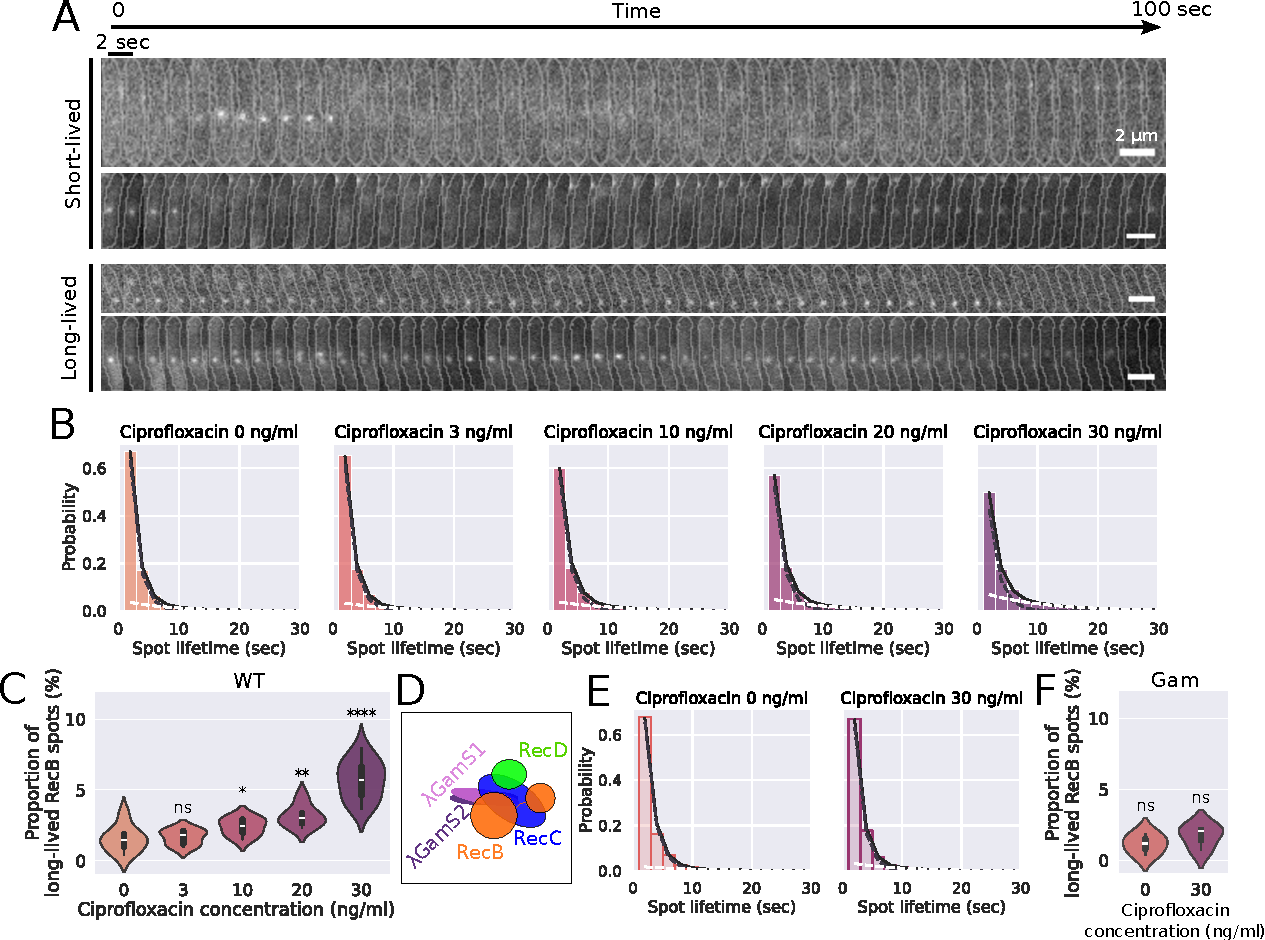
\includegraphics[width=.8\textwidth]{Figures/Fig2_RecB_lifetime.pdf}
    \caption{RecB spot lifetimes under ciprofloxacin exposure. \textbf{(A)} Example kymographs (2-sec interval, 100 sec total) of cells containing short- and long-lived RecB spots. \textbf{(B)} RecB spot lifetime histograms at 0, 3, 10, 20 and 30 ng/ml ciprofloxacin (bars), fitted with a bi-exponential decay model (black line, fit components shown as dashed lines). \ncells{66,764}. \nspots{170,138}. \textbf{(C)} RecB spot lifetime histograms (bars) for cells over-expressing the Gam protein, fitted with a bi-exponential decay model (black line, fit components shown as dashed lines). \ncells{8,812}. \nspots{18,698}. \textbf{(D)} Probability of a spot corresponding to a DSB-bound RecB molecule. Black dots show averages for individual datasets; the black line is the average between them, and the red dashed line shows the smallest lifetime at which RecB spots have a 95\% probability of being DSB-bound. \ncells{8,812}. \nspots{18,698}.}
    \label{Fig:lifetimes}
\end{figure*}

\begin{table}[htbp]
    \centering
    \caption{Parameters derived from the spot lifetime histogram fits (Figures \ref{Fig:lifetimes}B and \ref{Fig:lifetimes}C). The lifetime was calculated as the inverse of the fitted dissociation rate. Values are given as the median $\pm$ standard deviation over at least 3 independent datasets. \ncells{66,764}. \nspots{170,138}}
    \begin{tabular}{lllll}
        \toprule
        &  &  & \makecell{Lifetime\\(sec)} & \makecell{Population\\(\%)} \\
        Strain & \makecell{Cipro.} & Type &  &  \\
        \midrule
        \multirow[t]{10}{*}{WT} & \multirow[t]{2}{*}{0 ng/ml} & Short & 1.4 $\pm$ 0.2 & 98.2 $\pm$ 1.0 \\
        &  & Long & 9.5 $\pm$ 9.7 & 1.8 $\pm$ 1.0 \\
        \cline{2-5}
        & \multirow[t]{2}{*}{3 ng/ml} & Short & 1.5 $\pm$ 0.1 & 98.6 $\pm$ 0.3 \\
         &  & Long & 10.5 $\pm$ 1.3 & 1.4 $\pm$ 0.3 \\
        \cline{2-5}
        & \multirow[t]{2}{*}{10 ng/ml} & Short & 1.7 $\pm$ 0.2 & 97.6 $\pm$ 0.6 \\
        &  & Long & 13.7 $\pm$ 2.3 & 2.4 $\pm$ 0.6 \\
        \cline{2-5}
        & \multirow[t]{2}{*}{20 ng/ml} & Short & 1.6 $\pm$ 0.2 & 96.6 $\pm$ 0.8 \\
        &  & Long & 11.8 $\pm$ 2.1 & 3.4 $\pm$ 0.8 \\
        \cline{2-5}
        & \multirow[t]{2}{*}{30 ng/ml} & Short & 1.7 $\pm$ 0.2 & 94.5 $\pm$ 1.4 \\
        &  & Long & 13.3 $\pm$ 2.2 & 5.5 $\pm$ 1.4 \\
        \midrule
        \multirow[t]{4}{*}{Gam} & \multirow[t]{2}{*}{0 ng/ml} & Short & 1.7 $\pm$ 0.2 & 99.2 $\pm$ 0.4 \\
        &  & Long & 15.5 $\pm$ 9.1 & 0.8 $\pm$ 0.4 \\
        \cline{2-5}
        & \multirow[t]{2}{*}{30 ng/ml} & Short & 1.5 $\pm$ 0.1 & 98.2 $\pm$ 0.9 \\
        & & Long & 8.2 $\pm$ 1.8 & 1.8 $\pm$ 0.9 \\
        \bottomrule
        \end{tabular}
    \label{tab:fit_results}
\end{table}

% Gam
To determine whether short- or long-lived spots resulted from RecB binding to DSBs, we measured RecB spot lifetime in the presence and absence of ciprofloxacin while over-expressing the Gam protein of phage $\lambda$ from a plasmid. The Gam protein was previously shown to bind to the RecBCD complex by mimicking DNA double-strand ends \cite{Wilkinson2016}, and its overexpression is therefore expected to prevent RecBCD binding to DSBs. Accordingly, cells that expressed Gam and were exposed to high ciprofloxacin (30 ng/ml) showed little elongation compared to cells that did not overexpress Gam (Supp. Figure \ref{SIFig:Gam_cell_length}), indicating that most cells did not induce the SOS response, as a result of the inability of the RecBCD-Gam complex to bind to DSBs and load RecA. The resulting RecB spot lifetimes showed a similar distribution to the one obtained in the absence of ciprofloxacin (Supp. Figure \ref{SIFig:Gam_RecB_lifetimes_vs_WT}). This was confirmed by fitting the histogram with our bi-exponential decay model (Figure \ref{Fig:lifetimes}C), which found a proportion of long-lived spots in the presence of 30 ng/ml ciprofloxacin (1.8 $\pm$ 0.9\%, Table \ref{tab:fit_results}) equivalent to wild-type cells that were not exposed to ciprofloxacin (1.8 $\pm$ 1\%). The residual amount of long-lived RecB spots in the presence of Gam could be a result of residual DSB binding despite the presence of Gam. This residual binding could also explain the small increase in cell length observed in Gam-expressing cells under 30 ng/ml ciprofloxacin (Supp. Figure \ref{SIFig:Gam_cell_length}). Since Gam overexpression prevents RecB binding to DSBs, and specifically caused long-lived spots to disappear, we conclude that long-lived spots correspond to RecB molecules bound to a DSB (and we will refer to them as DSB-bound RecB throughout this article). Given that under Gam overexpression, 95\% of RecB spots had a lifetime shorter than 10 sec (Figure \ref{Fig:lifetimes}D), we considered any spot with a lifetime over 10 sec to be a DSB-bound RecB molecule. The appearance of short-lived spots in the presence of Gam is likely a result of a combination of short-lived DNA interactions and slow, confined diffusion of the RecBCD-Gam-Halo complex (Supp. Note \ref{note:spurious_spots} and Supp. Figure \ref{SIFig:displacement_simul}).

Using the Gam protein allowed us to identify DSB-bound RecB molecules as the longer-lived population in our bi-exponential fits of the RecB spot lifetime histograms. We determined that when it processes a DSB, RecB stays bound to it for 10 to 14 seconds on average, regardless of the ciprofloxacin concentration (Table \ref{tab:fit_results}). This is consistent with processing of DSBs by RecBCD taking place independently of the number of DSBs in the cell. In addition, to test whether the duration of ciprofloxacin exposure affected spot lifetimes, we performed separate fits at 15 min intervals for cells exposed to 30 ng/ml ciprofloxacin (Supp. Figure \ref{SIFig:RecB_lifetimes_timepoints}). The RecB spot lifetimes obtained were consistent with those reported in Table \ref{tab:fit_results} (10-15 sec for long-lived spots, and 1.5-2 sec for short-lived spots), indicating that RecB binding was not affected by the duration of ciprofloxacin exposure. This suggests that as expected, the presence of additional damage due to continuous exposure to ciprofloxacin does not influence the processing of DSBs by RecBCD

\subsection*{RecB dissociation time depends on its exonuclease activity}
% RecB binding time in the mutants
Since the duration of the RecB-DSB interaction was unaffected by the amount of DNA damage, we wondered if it was an intrinsic property of RecBCD processing, or if dissociation of the complex was triggered by the following step in the repair process, the loading of RecA on DNA. To assess this, we used the \dreca\ mutant, which lacks the RecA protein, and the \geneteneighty\ mutant, where RecB has lost its exonuclease activity, as well as its RecA loading activity. We imaged both strains in the presence and absence of ciprofloxacin (30 ng/ml), computed histograms of RecB spot lifetimes and fitted them with a bi-exponential decay model (Supp. Figure \ref{SIFig:mutants_biexp_fits}), from which we extracted the binding times of RecB on DSBs (Table \ref{tab:fit_mutants}). In the \dreca\ mutant, the DSB-binding lifetime of RecB was similar to the wild-type ($\sim$12 sec), both in the presence and absence of ciprofloxacin. This suggests that RecA loading by RecBCD does not play a role in triggering the dissociation of wild-type RecBCD from DNA. In contrast, \teneighty\ stayed bound to DSBs for longer on average than wild-type RecB ($\sim$16 to 19 sec), highlighting the importance of its exonuclease activity in dissociating from DNA. This could be due to the DNA strands threading through the RecBCD complex. The wild-type RecBCD digests the DNA strands as it translocates, which likely makes it easier to dissociate, for example through a short back-tracking motion. In contrast, \teneighty\ unwinds the DNA strands without digesting them, which would cause significant steric hindrance to dissociation.

% Table 2: RecB spot lifetime in the mutants
\begin{table}[htbp]
    \centering
    \caption{Parameters derived from the spot lifetime histogram fits for the \dreca\ and \geneteneighty\ strains (Supp. Figure \ref{SIFig:mutants_biexp_fits}). The lifetime was calculated as the inverse of the fitted dissociation rate. Values are given as the median $\pm$ standard deviation over at least 3 independent datasets. \ncells{56,131}. \nspots{177,646}.}
    \begin{tabular}{lllll}
        \toprule
        &  &  & \makecell{Lifetime\\(sec)} & \makecell{Population\\(\%)} \\
        Strain & Cipro. & Type &  &  \\
        \midrule
        \multirow[t]{4}{*}{\dreca} & \multirow[t]{2}{*}{0 ng/ml} & Short & 1.8 $\pm$ 0.2 & 96.6 $\pm$ 1.0 \\
        &  & Long & 13.0 $\pm$ 1.8 & 3.5 $\pm$ 1.0 \\
        \cline{2-5}
        & \multirow[t]{2}{*}{30 ng/ml} & Short & 2.1 $\pm$ 0.2 & 90.5 $\pm$ 3.4 \\
        &  & Long & 12.4 $\pm$ 3.5 & 9.5 $\pm$ 3.4 \\
        \midrule
        \multirow[t]{4}{*}{$recB_{1080}$} & \multirow[t]{2}{*}{0 ng/ml} & Short & 1.8 $\pm$ 0.2 & 97.4 $\pm$ 0.9 \\
        &  & Long & 16.7 $\pm$ 5.5 & 2.6 $\pm$ 0.9 \\
        \cline{2-5}
        & \multirow[t]{2}{*}{30 ng/ml} & Short & 2.1 $\pm$ 0.1 & 96.5 $\pm$ 0.7 \\
        &  & Long & 19.4 $\pm$ 7.1 & 3.5 $\pm$ 0.7 \\
        \bottomrule
    \end{tabular}
    \label{tab:fit_mutants}
\end{table}

% Rate of recruitment of RecB to DSBs
\subsection*{RecB binding can be used to estimate the rate of DSB formation}

\begin{figure}[htbp]
    \centering
    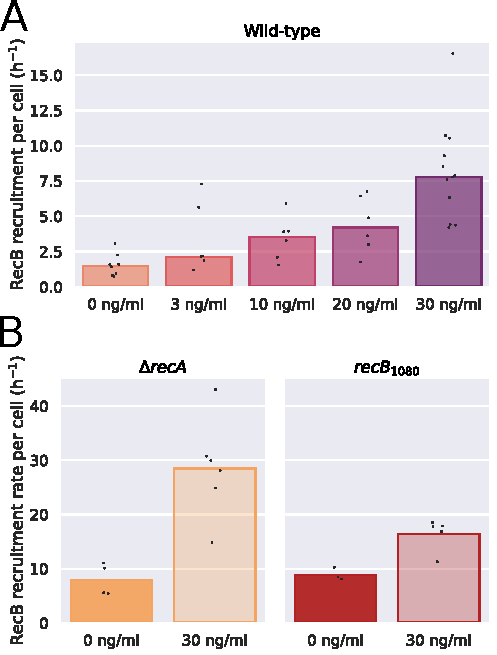
\includegraphics[width=.4\textwidth]{Figures/Fig3_RecB_recruitment.pdf}
    \caption{Recruitment of RecB to DSBs. \textbf{(A)} Recruitment rate of RecB to DSBs per cell at different ciprofloxacin concentrations. Black points show averages for individual datasets, and bars the median value between them. \ncells{66,764}. \nspots{170,138}. \textbf{(B)} Recruitment rate of RecB to DSBs per cell for the \dreca\ and \geneteneighty\ mutants. Black points show averages for individual datasets, and bars the median value between them. \ncells{23,540}. \nspots{99,891}.}
    \label{Fig:recruitment}
\end{figure}

% RecB recruitment in WT
Whereas the lifetime of RecB spots informs us on how long RecB stays bound to DSBs, the rate of appearance of spots can be used to estimate the rate of recruitment of RecB to DSBs under each DNA damage condition. To do so, we used the RecB spot lifetime histogram fits to estimate the total number of slow-dissociating spots per unit of time. Since we determined that the appearance of a slow-dissociating spot corresponds to the binding of RecB to a DSB, we could calculate the number of RecB recruitments to DSBs per cell per hour (Figure \ref{Fig:recruitment}A). We estimated that 1.3 $\pm$ 1.1 RecB molecules are recruited to DSBs per hour in the absence of ciprofloxacin. As expected, the recruitment rate of RecB scaled with ciprofloxacin concentration, up to 8.2 $\pm$ 3.6 RecB recruited to DSBs per hour at 30 ng/ml.

% RecB recruitment in mutants
Surprisingly, the rates of recruitment of RecB to DSBs in the \dreca\ and \geneteneighty\ mutants were higher than in the wild-type, both in the absence and in the presence of ciprofloxacin (Figure \ref{Fig:recruitment}B). In both cases, the rate of DSB formation is expected to be the same between the wild-type and the mutants as these mutations only affect the repair process downstream of DSB formation. Therefore, we hypothesise that this higher rate of RecB recruitment to DSBs is a result of multiple recruitment events on the same original DSB that cannot be repaired, as was previously reported in the case of the \dreca\ mutant \cite{Capaldo1975,Skarstad1993}. In the \geneteneighty\ mutant, RecB recruitment is higher than in WT cells, but equivalent (in the absence of ciprofloxacin) or lower (in the presence of 30 ng/ml ciprofloxacin) to the level of RecB recruitment in the \dreca\ mutant (Figure \ref{Fig:recruitment}B). This might reflect the ability of the \geneteneighty\ mutant to repair DSBs in a RecA-dependent manner, albeit with lower efficiency than wild-type cells (see Discussion).

% Part 3: Imaging RecA foci and filaments
\subsection*{Ciprofloxacin exposure induces formation of RecA filaments}
During DSB processing, RecBCD facilitates the loading of the RecA protein on ssDNA. To broaden our view of the repair process down\-stream of RecBCD, we imaged a tandem fusion of RecA with the fluorescent protein SYFP2, which was previously shown to preserve RecA functionality \cite{Wiktor2021}. Based on the fluorescence distribution in the cells (Supp. Figure \ref{SIFig:reca_structures}A), we identified three states of RecA: diffuse; forming a bright focus; or forming an elongated structure (called "filament" thereafter), which matches previous \emph{in vivo} observations of RecA \cite{Wiktor2021}. Because of the large diversity of shapes observed, particularly for RecA filaments, detecting RecA structures using rule-based algorithms was challenging. Therefore, we designed and trained a deep-learning algorithm capable of classifying individual cells based on the three types of spatial distributions cited above (Supp. Figures \ref{SIFig:object_class} and \ref{SIFig:reca_structures}B). In cells not exposed to ciprofloxacin, the RecA-associated fluorescence was mostly diffuse, and formed either a bright focus or a filament in $\sim$20\% of the cells. This is consistent with the expectation that RecA diffuses freely in the cell without DNA damage, and polymerises on DNA in the event of an endogenous DSB. After one hour of exposure, the proportion of cells that contained a RecA filament had increased to $\sim$40\% at 20 ng/ml ciprofloxacin, and $\sim$60\% at 30 ng/ml. RecA foci, on the other hand, formed rapidly following ciprofloxacin exposure (present in $\sim$40\% of the cells after 15 min of exposure to 30 ng/ml ciprofloxacin) and dissipated after $\sim$1 hour. Taken together, these results show that RecA foci are transient structures in the repair process that do not accumulate under high DNA damage, whereas RecA filaments accumulate under constant exposure to ciprofloxacin (see Discussion). They are also consistent with our observations of RecB recruitment rates per cell in the presence and absence of ciprofloxacin.

% Part 4: Colocalisation of RecB with the nucleoid
\subsection*{DSB-bound RecB colocalises with the bacterial nucleoid}

\begin{figure*}[htbp]
    \centering
    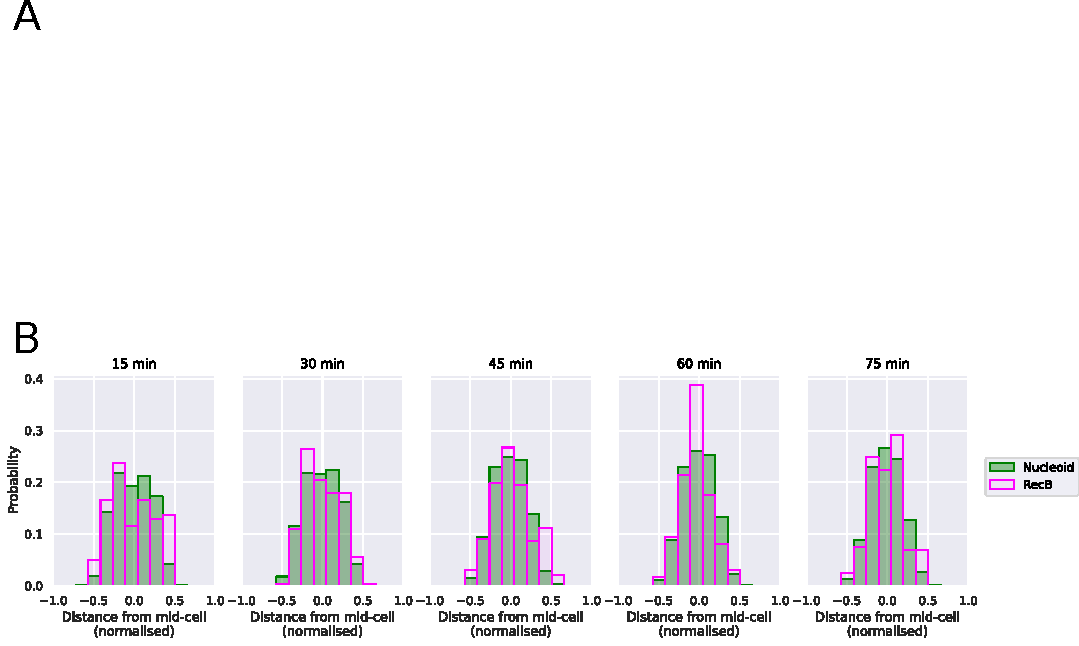
\includegraphics[width=.8\textwidth]{Figures/Fig4_nucleoid.pdf}
    \caption{Colocalisation of RecB spots with the bacterial nucleoid. \textbf{(A)} Representative images of cells (segmented outline in grey) showing the nucleoid (green) and RecB-associated fluorescence (magenta). RecB spots (indicated by arrows) are located in close proximity to the nucleoid. \textbf{(B)} Overlay of nucleoid density (green area) and position of DSB-bound RecB molecules (magenta bars) along the cell's long axis, for different ciprofloxacin concentrations (0 to 30 ng/ml). \ncells{24,014}. \nspots{79,969}. \nnucl{31,441}. \textbf{(C)} Representative overlay images of RecB-associated fluorescence (magenta) and the bacterial nucleoid (green) in the \dreca\ and \geneteneighty\ mutants. Segmented cell outline shown in grey. \textbf{(D)} Overlay of nucleoid density (green area) and position of DSB-bound RecB molecules (magenta bars) along the cell's long axis for the \dreca\ and \geneteneighty\ mutants at 0 and 30 ng/ml ciprofloxacin. \ncells{7,804}. \nspots{36,595}. \nnucl{11,215}.}
    \label{Fig:nucleoid}
\end{figure*}

% Nucleoid imaging
RecA loading on ssDNA triggers the SOS response, which inhibits cell division, leading to cell filamentation. Previous studies have reported that the SOS response also triggers compaction of the bacterial nucleoid \cite{Odsbu2014}. To see if this was the case for breaks induced by ciprofloxacin in our experimental conditions, we stained DNA using the Sytox Green dye. The use of a green dye allowed us to image RecB concomitantly, and to correlate the position of DSB-bound RecB molecules (defined as RecB spots with a lifetime $>$10 sec, see Figure \ref{Fig:lifetimes}D) with that of the nucleoid. In cells that were not exposed to ciprofloxacin, the nucleoid was often observed to be bi-lobed (Figure \ref{Fig:nucleoid}A), consistently with our previous observations \cite{Lepore2023}. After 60 min of exposure to ciprofloxacin, the cells appeared elongated, and the nucleoid was often compacted in the centre of the cell. As a result of nucleoid compaction, the total fraction of the cell occupied by the nucleoid decreased, from 40\% on average in untreated cells to 31\% in cells exposed to 30 ng/ml of ciprofloxacin for an hour (Supp. Figure \ref{SIFig:nucleoid_compaction}). In addition to the compaction, we observed that nucleoids were increasingly centred, and the cells elongated upon increasing exposure to ciprofloxacin, both in time and concentration (Supp. Figure \ref{SIFig:nucleoid_position}).

% Correlation of nucleoid and RecB spots
Long-lived RecB spots were found close to the nucleoid (Figures \ref{Fig:nucleoid}A and \ref{Fig:nucleoid}B). This proximity was observed at any time during the experiment (Supp. Figure \ref{SIFig:recb_nucleoid_timepoints}), suggesting that this proximity does not depend on the number of DSBs present in the cell. This observation strengthens our interpretation that long-lived spots are DSB-bound RecB molecules. Upon exposure to increasing ciprofloxacin concentrations, induction of the SOS response caused the cells to elongate significantly (from 3.1 $\pm$ 0.19 µm on average in the absence of ciprofloxacin to 5.5 $\pm$ 0.71 µm after 75 min of exposure to 30 ng/ml ciprofloxacin, Supp. Figure \ref{SIFig:Gam_cell_length}). Despite this, and because of compaction and centring, the nucleoid remained within $\sim$2 µm either side of the cell centre. The distribution of DSB-bound RecB molecules overlapped strongly with nucleoid density (Figure \ref{Fig:nucleoid}B), indicating that as the nucleoid was compacted, DSBs triggered RecB recruitment at the centre of the cell, where the nucleoid was located.

\subsection*{Nucleoid compaction requires RecA loading}
The spatial distribution of nucleoid density and DSB-bound RecB was affected in the \dreca\ and \geneteneighty\ mutants (Figures \ref{Fig:nucleoid}C and \ref{Fig:nucleoid}D). In the \dreca\ mutant, exposure to ciprofloxacin did not trigger nucleoid compaction and centring as in wild-type cells. This confirmed that nucleoid compaction under ciprofloxacin exposure requires RecA loading, and most likely the induction of the SOS response. Despite the absence of compaction, the nucleoid occupied a smaller fraction of the cell in the \dreca\ mutant after exposure to ciprofloxacin (Supp. Figure \ref{SIFig:mutants_nucleoid_compaction}). This can be attributed to the progressive degradation of the bacterial chromosome by the repeated cycles of RecBCD binding (Figure \ref{Fig:recruitment}B).

In the \geneteneighty\ mutant, the nucleoid often formed irregular shapes and small segregated regions in the cell (Figure \ref{Fig:nucleoid}C). This disorganisation was especially visible in the presence of 30 ng/ml ciprofloxacin. Furthermore, in the \geneteneighty\ mutant the nucleoid did not undergo compaction within the 75 min of our experiment (Supp. Figure \ref{SIFig:mutants_nucleoid_compaction}). This might reflect the less efficient RecA loading in this mutant, leading to different time dynamics of the SOS induction and either impaired or significantly delayed nucleoid compaction.

In both mutant strains, the localisation of DSB-bound RecB overlapped with the bacterial nucleoid (Figure \ref{Fig:nucleoid}D), similarly to the wild-type. In the \dreca\ mutant, addition of 30 ng/ml ciprofloxacin did not change the spatial distribution of nucleoid density or DSB-bound RecB. This result was expected, as \dreca\ cells were unable to induce the SOS response, and, therefore, did not undergo nucleoid compaction. In the \geneteneighty\ mutant in the absence of ciprofloxacin, both nucleoid density and DSB-bound RecB distributions were more centred than in wild-type cells, despite the nucleoid occupying the same fraction of the cell area (Supp. Figure \ref{SIFig:mutants_nucleoid_compaction}). This might be because of the slower growth rate of the \teneighty\ mutant resulting in a larger proportion of cells having a single centred nucleoid, rather than a bi-lobed nucleoid as seen in the wild-type and the \dreca\ mutant. Upon exposure of the \geneteneighty\ mutant to ciprofloxacin, the absence of change in the distribution of nucleoid density and DSB-bound RecB position reinforced the hypothesis that nucleoid compaction is impaired or delayed in this mutant.

